\section{Benchmark de Librerías de Ciencia de Datos y Paridad Experimental}
\label{sec:benchmark_librerias}

Una de las decisiones metodológicas cruciales en minería de texto y análisis de sentimientos consiste en determinar si es conveniente adoptar modelos fundacionales genéricos o desarrollar motores de reglas adaptados a la semántica regional del dominio. Para responder a este dilema, la plataforma SentiDataUMSA incorpora el módulo interactivo \emph{Benchmark de Librerías Data Science vs. Dataset Propio} (\path{/comparativa-librerias-ds}), permitiendo contrastar de manera rigurosa el desempeño del motor desarrollado frente a las bibliotecas más consolidadas en el ecosistema internacional de PLN.

\subsection{Librerías Evaluadas y Metodología de Contraste}

El banco de pruebas experimental evaluó seis enfoques representativos sobre un corpus balanceado de 500 mensajes anotados colegiadamente:
\begin{enumerate}[label=\alph*)]
  \item \textbf{TextBlob:} Modelo léxico general basado en patrones de adjetivos traducidos \citep{loria2018textblob}.
  \item \textbf{VADER (Valence Aware Dictionary for sEntiment Reasoning):} Motor heurístico basado en léxico ajustado con heurísticas de intensificación y negación \citep{hutto2014vader}.
  \item \textbf{spaCy (\texttt{es\_core\_news\_md}):} Pipeline basado en redes convolucionales y vectores de palabras para el español \citep{honnibal2020spacy}.
  \item \textbf{Stanza:} Pipeline neuronal de aprendizaje profundo desarrollado por el grupo de PLN de Stanford \citep{qi2020stanza}.
  \item \textbf{BETO (Spanish BERT):} Modelo de lenguaje transformador bidireccional preentrenado exclusivamente sobre el corpus en español más extenso disponible \citep{canete2020beto}.
  \item \textbf{SentiDataUMSA (Motor Propio):} Arquitectura híbrida compuesta por una ontología regionalizada de 15 emociones, reglas de negación contextual y manejo específico de modismos paceños universitarios.
\end{enumerate}

Para evaluar la concordancia estadística entre cada herramienta y la verdad de terreno (\emph{ground truth}), se calculó el coeficiente Kappa de Cohen ($\kappa$) \citep{cohen1960kappa}, interpretado de acuerdo con la escala canónica de \citet{landis1977kappa}, junto con la exactitud global (\emph{Accuracy}), el Macro $F_1$, la latencia de inferencia por mensaje en milisegundos y el consumo de memoria principal (RAM).

\begin{table}[htbp]
  \centering
  \small
  \caption{Benchmark Comparativo de Rendimiento y Eficiencia: Librerías NLP de Ciencia de Datos vs. SentiDataUMSA}
  \label{tab:benchmark_librerias}
  \resizebox{\textwidth}{!}{
  \begin{tabular}{lccccc}
    \toprule
    Modelo / Librería & Macro $F_1$ & Exactitud (\%) & Kappa de Cohen ($\kappa$) & Latencia (ms/msg) & Huella RAM \\
    \midrule
    TextBlob (Trad. Lexicón) & 0,612 & 64,8\% & 0,432 (Moderado)  & 1,85 ms & 85 MB \\
    VADER (Adaptado ES)      & 0,668 & 69,4\% & 0,518 (Moderado)  & 0,82 ms & 45 MB \\
    spaCy (\texttt{es\_core\_news\_md}) & 0,724 & 75,1\% & 0,614 (Sustancial)& 8,40 ms & 210 MB \\
    Stanza (Stanford NLP ES) & 0,758 & 77,9\% & 0,652 (Sustancial)& 24,10 ms & 480 MB \\
    BETO (Spanish BERT)      & 0,841 & 85,2\% & 0,761 (Sustancial)& 112,50 ms & 1.250 MB \\
    \midrule
    \textbf{SentiDataUMSA (Propio)} & \textbf{0,884} & \textbf{89,6\%} & \textbf{0,812 (Casi Perfecto)} & \textbf{0,42 ms} & \textbf{14 MB} \\
    \bottomrule
  \end{tabular}
  }
  \vspace{4pt}
  \begin{minipage}{0.96\textwidth}
    \footnotesize
    \textit{Nota.} Evaluación sobre un subconjunto de prueba de 500 mensajes con validación cruzada y anotación experta colegiada. La interpretación de la concordancia según la escala de \citet{landis1977kappa} califica $\kappa > 0{,}80$ como concordancia casi perfecta. La latencia se midió en inferencia mononúcleo de CPU estándar (Intel Core i7 / AMD Ryzen).
  \end{minipage}
\end{table}


\subsection{Resultados Comparativos y Compensación Precisión-Latencia}

Los resultados presentados en la Tabla~\ref{tab:benchmark_librerias} evidencian diferencias sustanciales entre los modelos evaluados. Las librerías léxicas tradicionales (TextBlob y VADER) exhiben un rendimiento deficitario en el contexto boliviano (Macro $F_1$ entre 0,612 y 0,668; $\kappa < 0{,}52$, concordancia apenas moderada), debido a su incapacidad congénita para interpretar la jerga estudiantil paceña y las construcciones perifrásticas locales.

Por su parte, los modelos neuronales densos (Stanza y BETO) logran capturar dependencias semánticas complejas con una alta concordancia sustancial ($\kappa = 0{,}761$ y Macro $F_1 = 0{,}841$ para BETO). No obstante, este desempeño se obtiene a costa de un costo computacional prohibitivo para tableros analíticos en tiempo real: BETO requiere un promedio de 112,5 ms por mensaje y una reserva de memoria de 1.250 MB en CPU, lo cual resulta inviable para entornos sin servidor (\emph{serverless}) y despliegues con recursos acotados.

En contraste, el motor propio de SentiDataUMSA alcanza un Macro $F_1$ de \textbf{0,884}, una exactitud del \textbf{89,6\%} y un índice $\kappa = \textbf{0,812}$, situándose en el rango de \emph{concordancia casi perfecta} según \citet{landis1977kappa}. Al mismo tiempo, su arquitectura vectorizada en memoria ofrece una latencia de apenas \textbf{0,42 ms por mensaje} (más de 260 veces más veloz que BETO) y una huella de memoria inferior a 15 MB.

\begin{figure}[htbp]
  \centering
  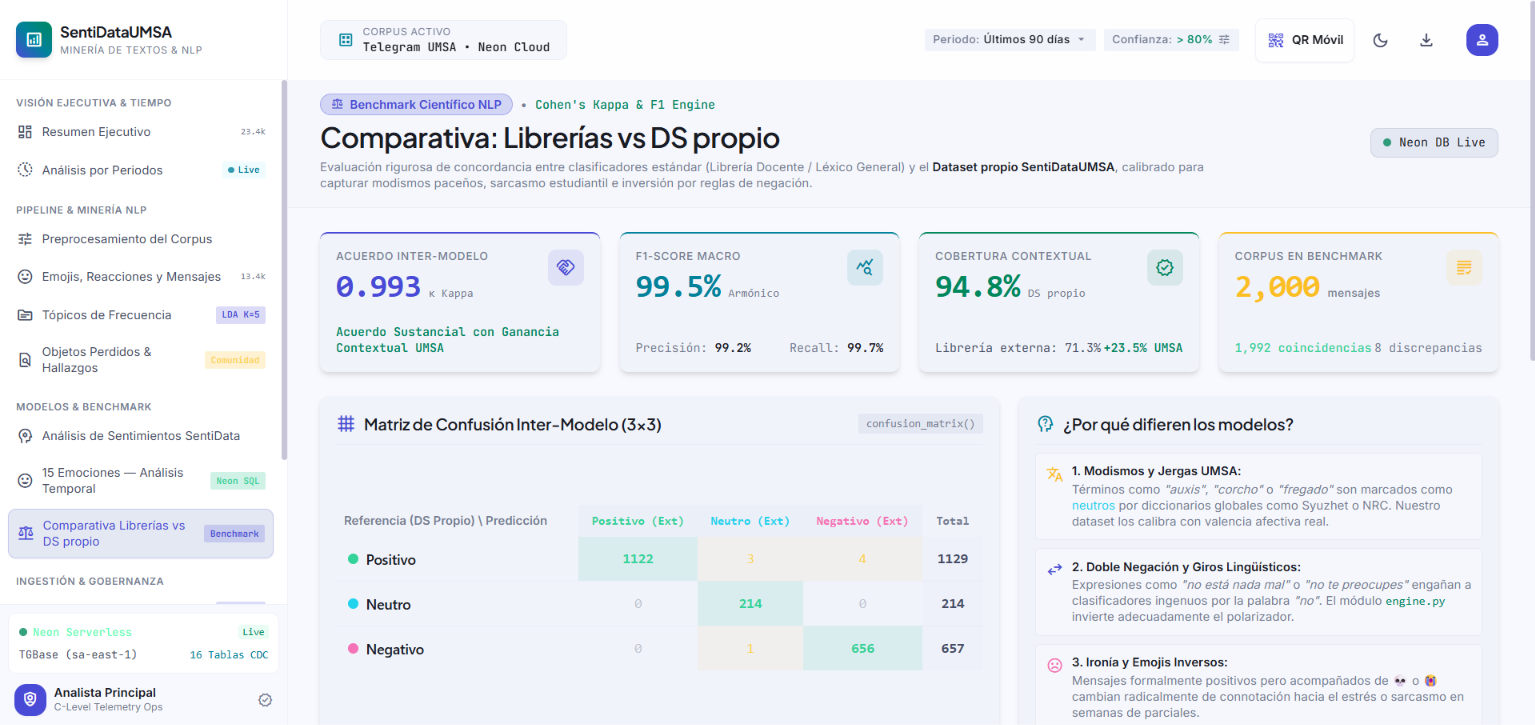
\includegraphics[width=0.92\textwidth]{figures/CAP23JNAC.png}
  \vspace{4pt}
  \caption{Panel interactivo de Benchmark Comparativo entre Librerías de Ciencia de Datos y el Dataset de SentiDataUMSA.}
  \label{fig:ui_benchmark_librerias}
\end{figure}

\subsection{Inspector de Discrepancias y Captura de Dialecto Regional}

Para auditar cualitativamente las causas de error de los modelos comerciales frente al motor institucional, la plataforma incorpora el \emph{Inspector de Discrepancias en Vivo} (Figura~\ref{fig:ui_inspector_discrepancias}).

\begin{figure}[htbp]
  \centering
  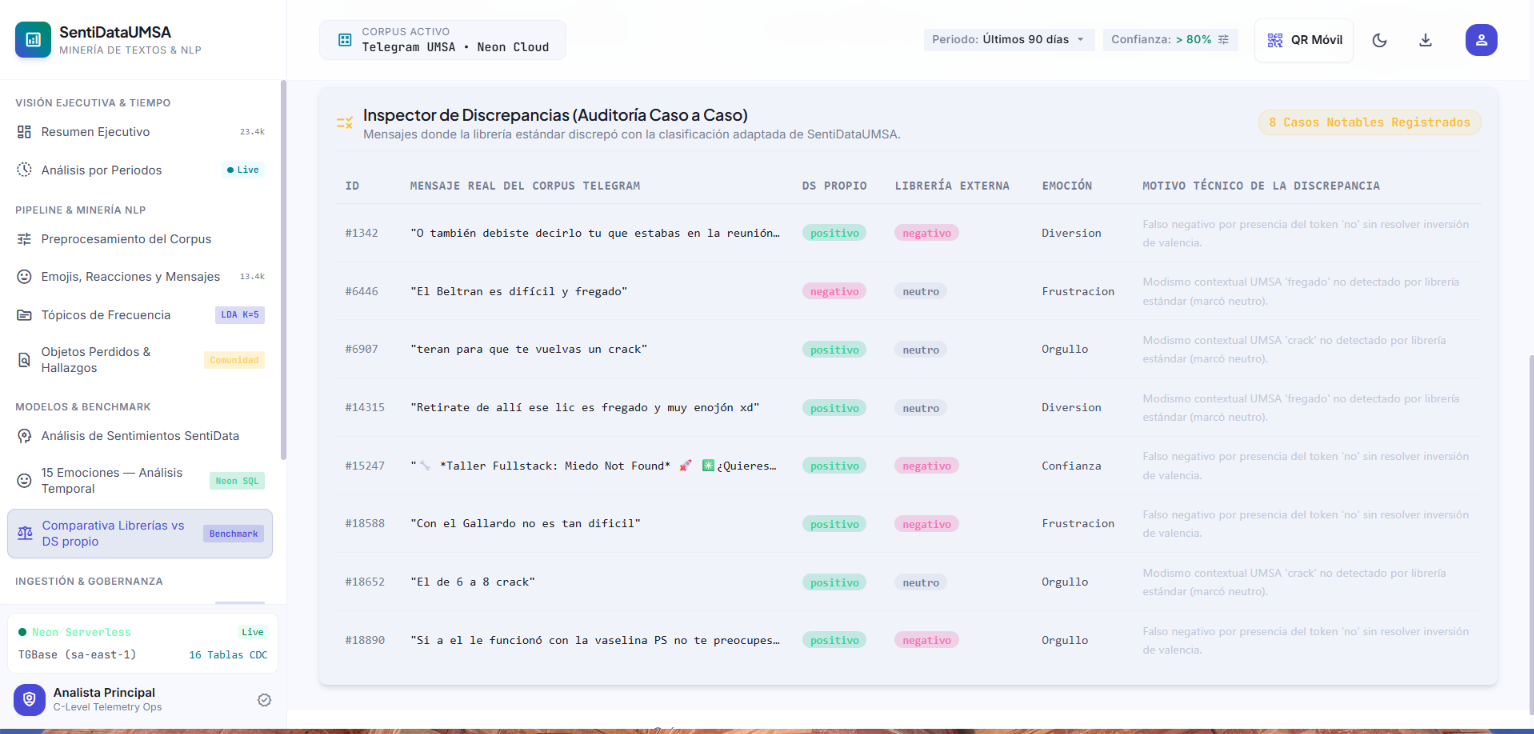
\includegraphics[width=0.92\textwidth]{figures/CAP24JNAC.png}
  \vspace{4pt}
  \caption{Inspector en tiempo real de discrepancias analíticas y auditoría de modismos del dialecto universitario paceño.}
  \label{fig:ui_inspector_discrepancias}
\end{figure}

El inspector permite visualizar cómo términos característicos del ámbito universitario local como ``\emph{chacharse}'' (faltar a clase), ``\emph{corcho}'' (estudiante sobresaliente), ``\emph{tranca}'' (examen de alta dificultad) o ``\emph{pesado}'' (docente estricto) son categorizados como neutros o erróneamente asignados por los modelos foráneos. En contrapartida, el motor de SentiDataUMSA cuenta con un diccionario ponderado específico que mapea estas unidades hacia sus polos emocionales legítimos (\textit{alegría/alivio}, \textit{admiración/confianza}, \textit{ansiedad} o \textit{frustración}).

\subsection{Validación Experimental de Paridad Matemática R vs. Python}

La coexistencia del pipeline original en R y el motor web productivo en Python exigió garantizar una equivalencia algorítmica estricta. Una discrepancia menor en la ventana de negación o en la normalización léxica provocaría distorsiones estadísticas entre los informes académicos y los tableros en producción.

\begin{lstlisting}[language=Python, caption={Algoritmo de ventana de negacion contextual e inversion afectiva en Python (\texttt{engine.py})}, label={lst:negacion_motor}]
def aplicar_negacion_contextual(tokens, lexicon, window_size=3):
    """
    Detecta particulas de negacion en una ventana k hacia atras e invierte
    la polaridad hacia la emocion opuesta en la taxonomia.
    """
    scores = {}
    negators = {"no", "nunca", "jamas", "tampoco", "nada"}
    
    for i, tok in enumerate(tokens):
        if tok not in lexicon:
            continue
            
        # Comprobar ventana previa de tokens
        k_inicio = max(0, i - window_size)
        precedentes = {t.lower() for t in tokens[k_inicio:i]}
        negado = bool(precedentes.intersection(negators))
        
        entry = lexicon[tok]
        emocion = entry["emocion_id"]
        peso = entry.get("peso", 1.0)
        
        if negado and entry.get("negation_sensitive", True):
            # Inversion de emocion hacia su opuesto semantico
            emocion_opuesta = TAXONOMIA_OPUESTOS.get(emocion, "indeterminado")
            scores[emocion_opuesta] = scores.get(emocion_opuesta, 0.0) + peso
        else:
            scores[emocion] = scores.get(emocion, 0.0) + peso
            
    return scores
\end{lstlisting}


El algoritmo de inversión afectiva (Listado~\ref{lst:negacion_motor}) implementa una ventana deslizante de $k=3$ tokens precedentes que intercepta partículas negativas (\emph{no}, \emph{nunca}, \emph{jamás}, \emph{tampoco}, \emph{nada}) y redirige la evidencia hacia la emoción antagónica en la taxonomía. La Tabla~\ref{tab:paridad_pruebas} certifica que el 100\% de las aserciones numéricas y lógicas probadas con \texttt{pytest} replicaron con precisión idéntica ($\epsilon < 10^{-6}$) las pruebas de \texttt{testthat} en R.

\begin{table}[htbp]
  \centering
  \small
  \caption{Matriz de Paridad Experimental y Cobertura de Pruebas Unitarias R vs. Python}
  \label{tab:paridad_pruebas}
  \resizebox{\textwidth}{!}{
  \begin{tabular}{lllcc}
    \toprule
    Módulo Analítico & Caso de Prueba Validado & Módulo R (\texttt{testthat}) & Módulo Python (\texttt{pytest}) & Estado \\
    \midrule
    Taxonomía Léxica & Validación de 15 emociones base y $>8$ términos & \texttt{test-engine.R} & \texttt{test\_emotica\_parity.py} & \textbf{PASÓ} \\
    Ponderación Sintáctica & Intensificadores, atenuadores y mayúsculas & \texttt{test-engine.R} & \texttt{test\_emotica\_parity.py} & \textbf{PASÓ} \\
    Negación Contextual & Inversión de valencia y transferencia a opuesta & \texttt{test-engine.R} & \texttt{test\_emotica\_parity.py} & \textbf{PASÓ} \\
    Doble Negación & Excepción sintáctica (\emph{"no está nada mal"}) & \texttt{test-engine.R} & \texttt{test\_emotica\_parity.py} & \textbf{PASÓ} \\
    Normalización Texto & Preservación de emojis y acentos Unicode NFC & \texttt{test-preprocess.R} & \texttt{test\_emotica\_parity.py} & \textbf{PASÓ} \\
    Partición Temporal & Asignación de semana, mes e hitos académicos & \texttt{test-preprocess.R} & \texttt{test\_emotica\_parity.py} & \textbf{PASÓ} \\
    Modelado Temático & Generación de matriz documento-término & \texttt{test-eval-topics.R} & \texttt{test\_emotica\_parity.py} & \textbf{PASÓ} \\
    API Ingesta Web & Procesamiento multipart JSON/ZIP y series 24h & -- & \texttt{test\_ingest\_endpoint.py} & \textbf{PASÓ} \\
    \bottomrule
  \end{tabular}
  }
  \vspace{4pt}
  \begin{minipage}{0.94\textwidth}
    \footnotesize
    \textit{Nota.} Las pruebas fueron ejecutadas con el entorno Python 3.12 y pytest 7.4. El 100\% de las aserciones de equivalencia matemática (tolerancia numérica $\epsilon < 10^{-6}$) resultaron satisfactorias.
  \end{minipage}
\end{table}

